\documentclass[10pt,aspectratio=1610]{beamer} % use option aspectratio=169 or 1610 for wide slides
% Note: For online presentations via Zoom use the ratio of the screen you want to share
\usetheme{Rochester}

% load syscop style
\usepackage{style/syscop}

%--------------------------------------------------
% TITLE
%--------------------------------------------------

% NOTE: what's in [ ] goes to footer for the fields title, author and date
\title[Not So Short Report on Riccati Solver]{\huge Not So Short Report on Riccati Solver}


%--------------------------------------------------
% Useful packages
%--------------------------------------------------

\usepackage{amsthm}
\usepackage{cite}
\usepackage{amsmath,amssymb,amsfonts}
\usepackage{graphicx}
\usepackage{textcomp}
\usepackage{xcolor}
\usepackage{optidef}
\usepackage{makecell}
\usepackage{booktabs}
\usepackage{multirow}
\usepackage{diagbox}
\usepackage{indentfirst}
\usepackage{float}
\usepackage{algorithm}
\usepackage{algpseudocode}
\usepackage{nicematrix}
\usepackage{acronym}
\usepackage{hyperref}

\begin{document}

\InsertTitle

\begin{frame}
    \frametitle{Quick walkthrough}
    A quick walkthrough on the report topics:
    \begin{itemize}
        \item Riccati-based primal regularizations
        \item Mehrotra probing instead of predictor-corrector
        \item Indefinite QP dataset from tracking OCPs (regulators)
        \item Numerical results
        \item Issues on time-optimal indefinite QPs
    \end{itemize}
\end{frame}

% Ensure \usepackage{amsmath} is included in your document preamble
\begin{frame}
    \frametitle{Schur complement reduced KKT system}
    Suppose an OCP QP problem solved by IPM.\\
    After Shur complement, the KKT system can be written as:
    \begin{equation}
        \begin{bmatrix}
        \tilde{H}^i & F^\top \\
        F & 0
        \end{bmatrix}
        \begin{bmatrix}
        \Delta y \\
        \Delta \pi
        \end{bmatrix} = -
        \begin{bmatrix}
        \tilde{r}_{\mathrm{stat}}^i \\
        r_{\mathrm{eq}}^i
        \end{bmatrix},
        \label{eq:schur_comp_KKT}
    \end{equation}
    where the $\tilde{H}^i = H + G^\top T_i^{-1}\Lambda_i G$ 
    and $\tilde{r}_{\mathrm{stat}}^i = r_{\mathrm{stat}}^i - G^\top T_i^{-1} ( \Lambda_i r_{\mathrm{ineq}}^i - r_{\mathrm{comp}}^i )$. \\
    \vspace{0.5cm}
    With the null space method as the $\Delta y = Y\Delta y_y + Z\Delta y_z$, 
    the Schur complement reduced KKT system follows as:
    \begin{equation}
        \tilde{M}^i \Delta y_z = - (Z^\top \tilde{r}_{\mathrm{stat}}^i - Z^\top \tilde{H}^i Y \Delta y_y)
        \label{eq:schur_comp_KKT_reduced}
    \end{equation}
    where $\tilde{M}^i = Z^\top \tilde{H}^i Z$ is the reduced Hessian. $\Delta y_y = (FY)^{-1}r_{\mathrm{eq}}^i$.

\end{frame}

\begin{frame}
    \frametitle{Riccati recursion as explicit L$^\top$DL decomposition}
    Riccati recursion can be regarded as an explicit L$^\top$DL decomposition of reduced Hessian $\tilde{M}^i$\\
    \begin{algorithm}[H]
    \caption{Backward Pass of Riccati Recursion}
    \label{alg:riccati_recursion}
    \begin{algorithmic}[1]
    \State\textbf{Initialize:} $P_N \gets \tilde{Q}_N$, $p_N \gets \tilde{r}_{\mathrm{stat}, x}^N$
    \Statex 
    \For{$k = N-1$ \textbf{down to} $0$}
        \State $\tilde{M}_k \gets \tilde{R}_k + B_k^\top P_{k+1} B_k$
        \State $\Gamma_k \gets \tilde{S}_k + B_k^\top P_{k+1} A_k$
        \State $K_k \gets -\tilde{M}_k^{-1} \Gamma_k$
        \State $k_k \gets -\tilde{M}_k^{-1} \left(\tilde{r}_{\mathrm{stat}, u}^k + B_k^\top (P_{k+1} r_{\mathrm{eq}}^k + p_{k+1})\right)$
        \State $P_k \gets \tilde{Q}_k + A_k^\top P_{k+1} A_k - \Gamma_k^\top K_k$
        \State $p_k \gets \tilde{r}_{\mathrm{stat}, x}^k + A_k^\top (P_{k+1} r_{\mathrm{eq}}^k + p_{k+1}) + \Gamma_k^\top k_k$
    \EndFor
    \end{algorithmic}
    \end{algorithm}
    Where $\tilde{M}_k$ is the block reduced Hessian at stage $k$.
\end{frame}

\begin{frame}
    \frametitle{Failing of minimal perturbation on block reduced Hessian 1/2}
    Assume $\tilde{M}_k$ has only one negative eigenvalue $\lambda_j$, and the corresponding eigenvector is $v_j$.

    The minimum perturbation strategy is applied as:
    \begin{equation}
        E_k = (-\lambda_{j}+\epsilon) v_j v_j^\top,
    \end{equation}
    where the $\epsilon$ is a positive value to ensure the positive definiteness of the regularized reduced Hessian block. 

    \vspace{0.5cm}

    By Sherman-Morrison formula, the inverse of the regularized reduced Hessian block can be expressed as:
    \begin{align*}
        (\tilde{M}_k + E_k)^{-1} &= \tilde{M}_k^{-1} + \frac{\lambda_j-\epsilon}{\epsilon \lambda_j} v_j v_j^\top \\
                                &= \tilde{M}_k^{-1} + (\frac{1}{\epsilon} - \frac{1}{\lambda_j}) v_j v_j^\top,
    \end{align*}

\end{frame}

\begin{frame}
    \frametitle{Failing of minimal perturbation on block reduced Hessian 2/2}
    the update of cost-to-go matrix $P_k$ follows as:
    \begin{align}
        P_k &= \tilde{Q}_k + A_k^\top P_{k+1} A_k - \Gamma_k^\top K_k \notag \\
            &=\tilde{Q}_k + A_k^\top P_{k+1} A_k - \Gamma_k^\top \tilde{M}_k^{-1} \Gamma_k - (\frac{1}{\epsilon} - \frac{1}{\lambda_j}) \Gamma_k^\top v_j v_j^\top \Gamma_k \notag \\
            &= P_k^{\mathrm{unmod}} - (\frac{1}{\epsilon} - \frac{1}{\lambda_j}) \Gamma_k^\top v_j v_j^\top \Gamma_k,
    \end{align}
    Consequently, the reduced Hessian block $\tilde{M}_{k-1}$ at the previous stage as:
    \begin{equation}
        \tilde{M}_{k-1} = \tilde{M}_{k-1}^{\mathrm{unmod}} - (\frac{1}{\epsilon} - \frac{1}{\lambda_j}) z_j z_j^\top,
    \end{equation}
    where $z_j = B_{k-1}^\top \Gamma_k^\top v_j$ is a column vector.
\end{frame}

\begin{frame}
    \frametitle{Proposed Riccati-based primal regularization}
    This issue reveals two insights in Riccati-based regularization:
    \begin{itemize}
        \item Avoid minimum perturbation on block reduced Hessian.
        \item The cost-to-go matrix $P_k$ should also be considered for regularization.
    \end{itemize}

    \vspace{0.5cm}

    We have proposed/attempted following Riccati-based primal regularizations:
    \begin{itemize}
        \item PM\_STAGE\_MIRROR: 

        For each stage $k$, 
        mirror $P_k$;
        compute $\tilde{M}_{k-1} = R_k + B^\top_k P_k^{reg}B_k$; 
        then mirror $\tilde{M}_{k-1}$.
        \item PM\_STAGE\_GMW: 

        Use GMW to substitute mirror in PM\_STAGE\_MIRROR.
        \item INERTIA\_CORRECTION: \

        Add constant value to full Hessian diagonally when Choleksky decomposition fails.

        Iterate until it succeeds, adapting same value update strategy in IPOPT.

    \end{itemize}

\end{frame}

\begin{frame}
    \frametitle{Mehrotra probing}
    According to the paper \cite{nocedalAdaptiveBarrierUpdate2009a} from Nocedal et al.
    Mehrotra probing could be a better strategy than predictor-corrector to update the barrier parameter $\tau$ in indefinite cases.

    \vspace{0.2cm}

    The residuals are defined as:
    \begin{equation}
        \begin{bmatrix}
		r_{\mathrm{stat}}^i \\
		r_{\mathrm{eq}}^i \\
		r_{\mathrm{ineq}}^i \\
		r_{\mathrm{comp}}^i
		\end{bmatrix}
        =
		\begin{bmatrix}
            Hy_i + g + F^\top \pi_i + G^\top \lambda_i \\
            Fy_i - b \\
            Gy_i + t_i - d \\
            T_i \Lambda_i \mathbf{1} - \sigma_i \mu_i \mathbf{1}
        \end{bmatrix}
        ,
\end{equation}
With $\sigma_i = \left( \frac{\mu_i^{\mathrm{aff}}}{\mu_i} \right)^3$, and the $\mu_i$ and $\mu_{\mathrm{aff}}^i$ are defined as:
\begin{equation}
    \mu_i = \frac{t_i^\top \lambda_i}{m},
\end{equation}

\begin{equation}
    \mu_i^{\mathrm{aff}} = \frac{(t_i + \alpha_{p,\mathrm{aff}}^i \Delta t_{\mathrm{aff}}^i)^\top (\lambda_i + \alpha_{d,\mathrm{aff}}^i \Delta \lambda_{\mathrm{aff}}^i)}{m},
\end{equation}

where $m$ is the number of inequality constraints.
\end{frame}

\begin{frame}{Step Size Selection: FTB and Funnel line search}
% ---------- Top: FTB ----------
\textbf{\textcolor{blue!60!black}{1. FTB scaling}}\quad
$\tau=1-\min(10^{-7},\mu)$, applied to $\alpha_p,\alpha_d$ each (steps back from the boundary to keep $\lambda,s>0$):
\[
\alpha \leftarrow
\begin{cases}
\alpha\big[(1-\alpha)\,0.99+\alpha\,\tau\big], & \alpha<1\\
\alpha, & \alpha=1
\end{cases}
\]
 
\vspace{0.4em}
% ---------- Bottom: acceptance ----------
\textbf{\textcolor{blue!60!black}{2. Acceptance \cite{kiesslingUnifiedFunnelRestoration2025}}}\quad (else $\alpha_p\!\leftarrow\!\beta\alpha_p$)
\begin{itemize}
  \item \textbf{In funnel?}\ \ $\theta^+\le\theta_{\max}$
  \item \textbf{Switching}\ \ $\alpha_p(-\rho)>\kappa_{s}\theta^2$\ ?
  \begin{itemize}
    \item[$\rightarrow$] \textbf{f-step} (Armijo): $\ f^+\le f+\gamma\alpha_p\rho$
    \item[$\rightarrow$] \textbf{h-step} (reduce $\theta$): $\ \theta^+\le \kappa_{h}\theta_{\max}$,\quad then shrink
    \[
      \theta_{\max}\leftarrow\max\big(\tfrac{\theta_{\max}+\theta^+}{2},\kappa_{m}\theta_{\max}\big)
    \]
  \end{itemize}
\end{itemize}
Where $\theta=\|c\|$ (constraint violation, bound $\theta_{\max}$), $\rho=\nabla f^\top d,\ d=(\Delta x,\Delta u,\Delta s)$.

\end{frame}



\begin{frame}
    \frametitle{Local quadratic convergence rate}
    The Riccati-based primal regularization will not modify the Hessian when converging to the local solution, i.e. LHS coincides with that of Newton step,
    \begin{lemma}
    Under isolated minimizers, LICQ and strict complementarity, given the sequence $\{W^i\}$ constructed by the algorithm, as \{$(y^i, \lambda^i)$\} $\rightarrow$ $(y^*, \lambda^*)$,
    $W^i = \tilde{M}^i = Z^\top \tilde{H}^i Z \succ 0$ for all $i$ sufficiently large.
    \end{lemma}
    Mehrotra probing will still guarantee the $\sigma_i$ $\mu_i$ = O($||\delta^N||^4$), i.e. RHS will approach that of Newton step.

    \vspace{0.2cm}

    With appropriate step size selection, the local quadratic convergence rate is proved.
\end{frame}

\begin{frame}
    \frametitle{Indefinite QP dataset: Generate and Collect}
    The indefinite QPs refers to QPs with indefinite reduced Hessian.

    \vspace{0.5cm}

    We generate a dataset of indefinite sub QPs from tracking OCPs (regulators) with acados, with two steps:
    \begin{enumerate}
        \item Generate: Applying PROJECT, MIRROR or Gauss-Newton approximation to generate iterates on an OCP problem;
        \item Collect: Loading the generated iterates for linearization in SQP and collecting the indefinite sub QPs.
    \end{enumerate}

    \vspace{0.3cm}

    We apply this pipeline on 8 different OCP problems, and collect 155 indefinite QPs in total.
\end{frame}

\begin{frame}
    \frametitle{Indefinite QP dataset: quick overview of OCP problems}
    \centering
    \begin{tabular}{l l c c c}
        \hline
        \textbf{Problem} & $n_x$ & $n_u$ & $N$ \\
        \hline
        Pendulum     & 4  & 1 & 20 \\
        Acrobot      & 4  & 2 & 15 \\
        Dubins car parking   & 3  & 2 & 25 \\
        Furuta       & 4  & 1 & 20 \\
        Flying robot & 6  & 4 & 30 \\
        robot arm    & 6  & 3 & 30 \\
        crane        & 6  & 2 & 35 \\
        moonlander   & 6  & 2 & 30 \\
        \hline
    \end{tabular}

    \vspace{0.5cm}

    All the OCP problems are formulated as regulators.
\end{frame}

\begin{frame}
    \frametitle{Scatter plot of indefiniteness and coverage}
    \begin{figure}[H]
        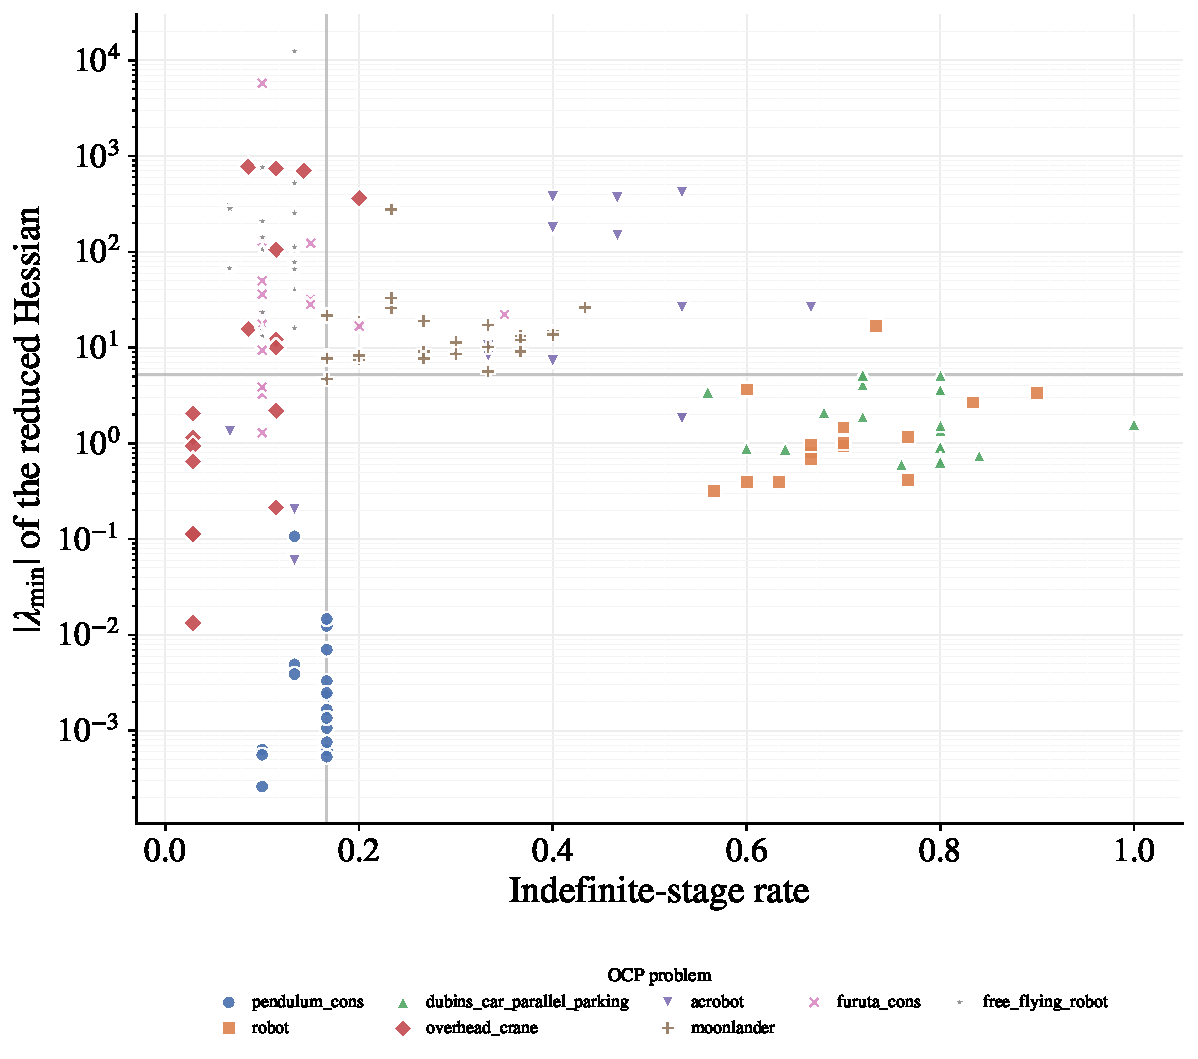
\includegraphics[width=0.65\textwidth]{results/indefiniteness_coverage_scatter.pdf}
        \label{fig:indefinite_qp_dataset_analysis}
    \end{figure}
\end{frame}

\begin{frame}
  \frametitle{Distribution of indefiniteness and coverage}
  \begin{columns}[T]
    \begin{column}{0.5\textwidth}
      \centering
      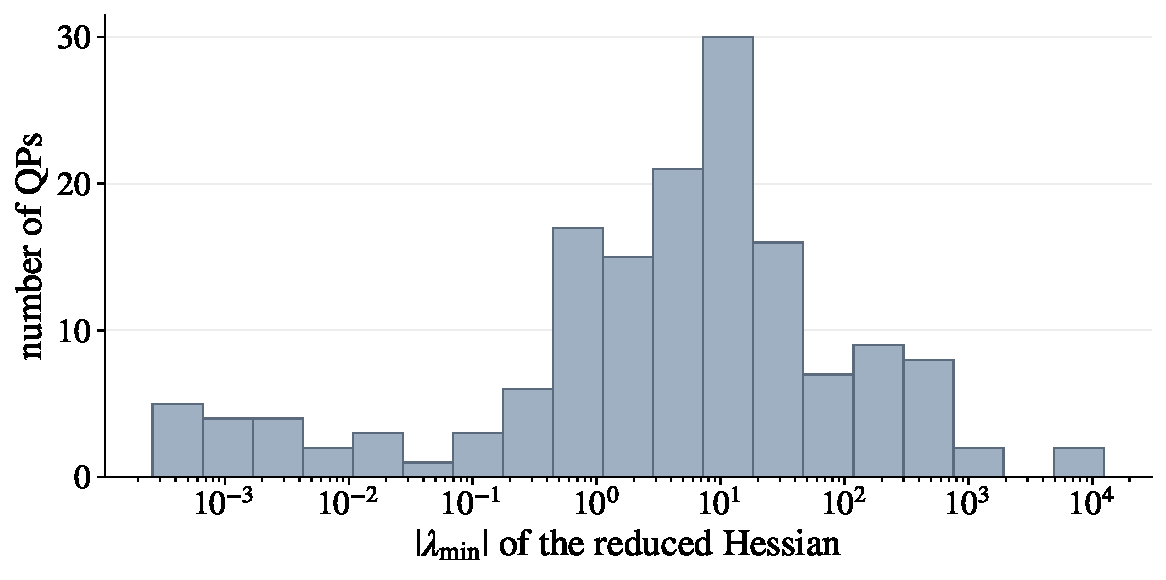
\includegraphics[width=\linewidth]{results/indefiniteness_coverage_depth.pdf}
      \small How indefinite: $|\lambda_{\min}|$ of the reduced Hessian
    \end{column}
    \begin{column}{0.5\textwidth}
      \centering
      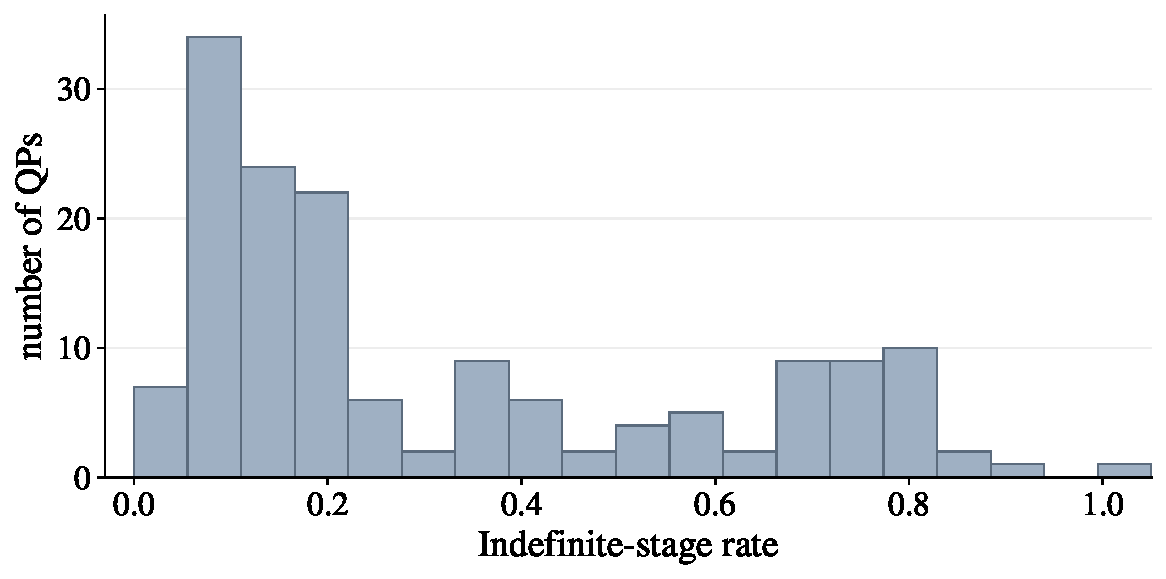
\includegraphics[width=\linewidth]{results/indefiniteness_coverage_breadth.pdf}
      \small How often: fraction of stages that are indefinite
    \end{column}
  \end{columns}
  \vspace{1em}
\end{frame}

\begin{frame}
  \frametitle{Stage indefiniteness source}
    \begin{figure}[H]
        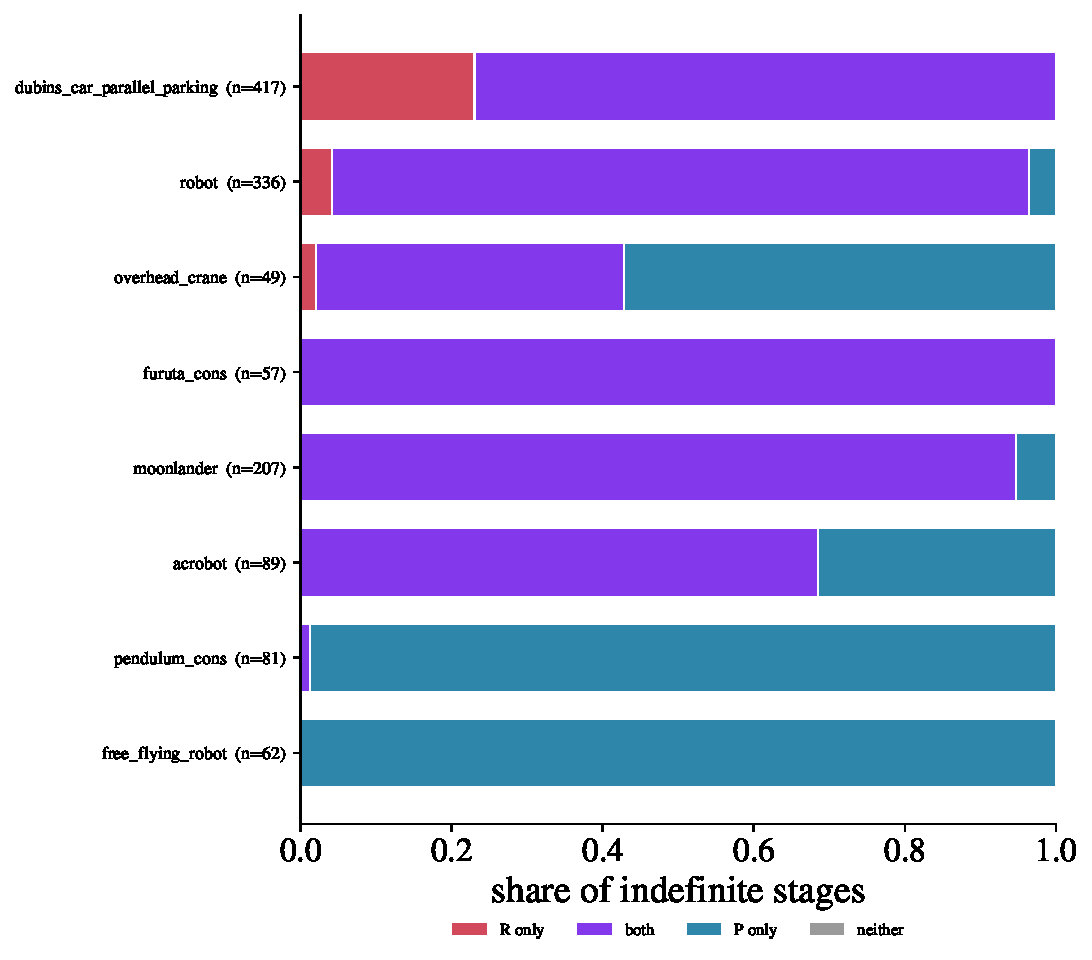
\includegraphics[width=0.65\textwidth]{results/stage_indefiniteness_signature.pdf}
    \end{figure}
\end{frame}

\begin{frame}
    \frametitle{Numerical results: Setup}
    We implemented a Riccati-based IPM solver in python, which produces similar iteration behavior as HPIPM in convex QPs\\

    \vspace{0.2cm}

    We compare the following regularizations on the indefinite QP dataset:
    \begin{itemize}
        \item PROJECT\_H: Do Project on full Hessian when reduced Hessian is indefinite
        \item MIRROR\_H: Do Mirror on full Hessian when reduced Hessian is indefinite
        \item PM\_STAGE\_MIRROR
        \item PM\_STAGE\_GMW
        \item INERTIA\_CORRECTION
        \item PRECOMPUTE: Precompute the regularization with PROJECT on the full Hessian before schur complement, and use it for indefinite reduced Hessian
    \end{itemize}

    \vspace{0.2cm}

    We also use IPOPT as a reference solver for indefinite QPs.

    \vspace{0.2cm}

    For tolerance, we set tolerance for $r_{\mathrm{stat}}$ and $r_{\mathrm{comp}}$ to $10^{-6}$, $r_{\mathrm{eq}}$ and $r_{\mathrm{ineq}}$ to $10^{-8}$.
\end{frame}

\begin{frame}
    \frametitle{Numerical results: iteration profile}
    \begin{figure}
        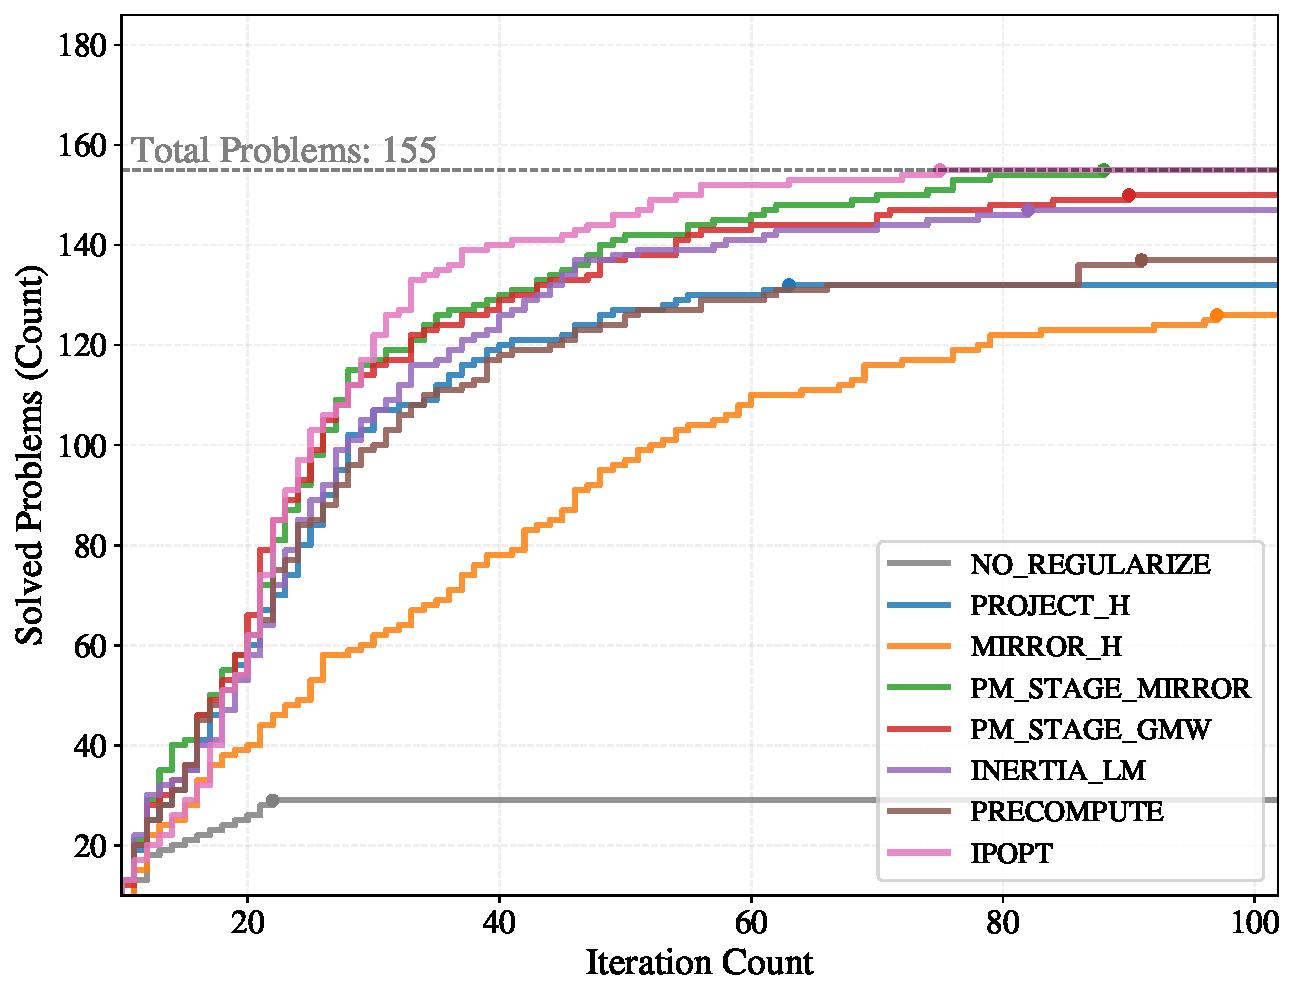
\includegraphics[width=0.7\textwidth]{results/iteration_qp_results_riccati.pdf}
    \end{figure}
\end{frame}

\begin{frame}
    \frametitle{Numerical results: flop proxy}
    In order to estimate the flop counting, we take one modified Cholesky factorization on block reduced Hessian as the unit, i.e.
    \begin{equation*}
        \mathrm{unit} \approx \frac{1}{3} n_u^3 \mathrm{,}
    \end{equation*}
    where $n_u$ is the control dimension.
    \vspace{0.2cm}

    The flops of eigenvalue decomposition is usually regarded as $9n^3$ \cite{verschuerenTimeoptimalRaceCar2016b}, 
    which is 27 units if modifying the block reduced Hessian.
\end{frame}

\begin{frame}
    \frametitle{Numerical results: box plot of flops with proxy}
    \begin{figure}
        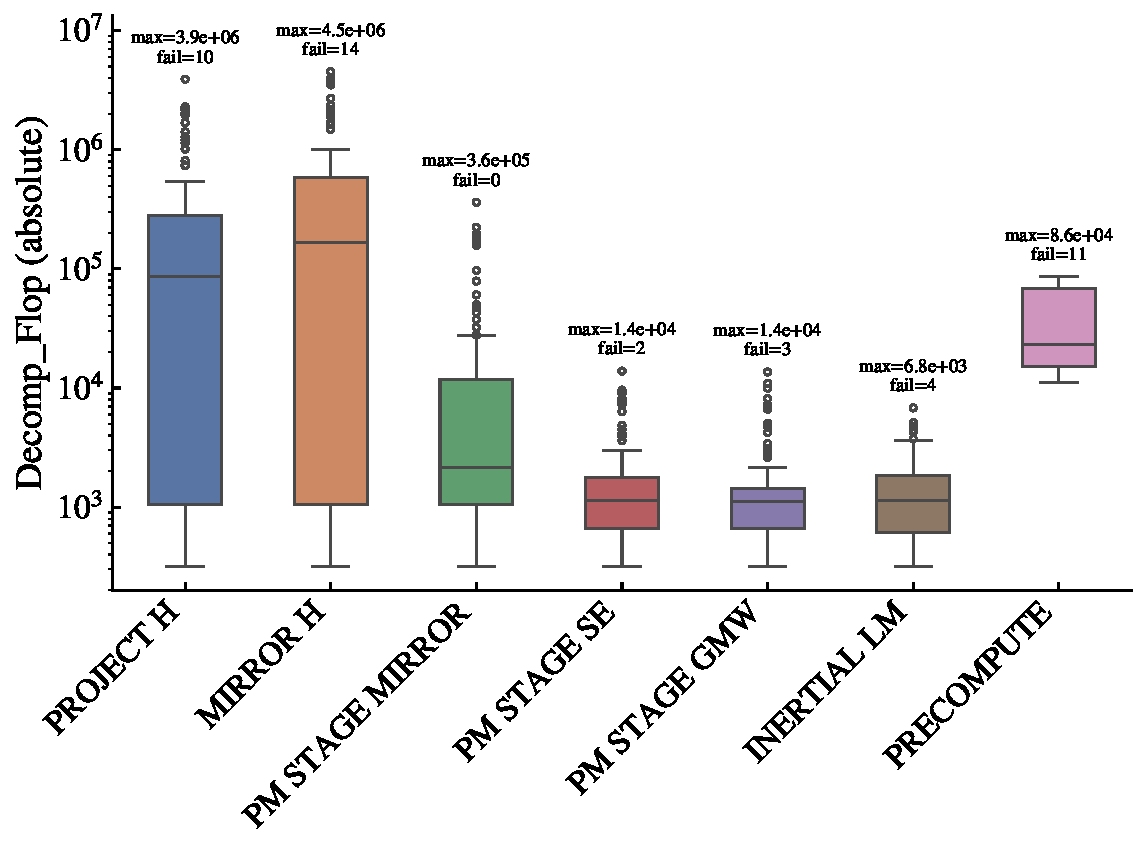
\includegraphics[width=0.7\textwidth]{results/decomp_flop_worstcase_qp_results_riccati.pdf}
    \end{figure}
\end{frame}

\begin{frame}
    \frametitle{Issues on time-optimal indefinite QPs}
    The current method does not work well on time-optimal indefinite QPs.\\
    \vspace{0.2cm}
    We collect 4 time-optimal OCPs and corresponding 84 indefinite QPs:

    \vspace{0.5cm}

    \begin{tabular}{l l c c c c}
        \hline
        \textbf{Problem} & $n_x$ & $n_u$ & $N$ & $T_f$\\
        \hline
        Pedulum             & 5  & 1 & 50  & 1.0\\
        Dubins car parking  & 4  & 2 & 50  & 3.0\\
        Dubins car obstacle & 4  & 2 & 25  & 5.0\\
        hangglider          & 7  & 2 & 100 & 1.0\\
        \hline
    \end{tabular}
\end{frame}

\begin{frame}
    \frametitle{Issues on time-optimal indefinite QPs}
    \begin{figure}
        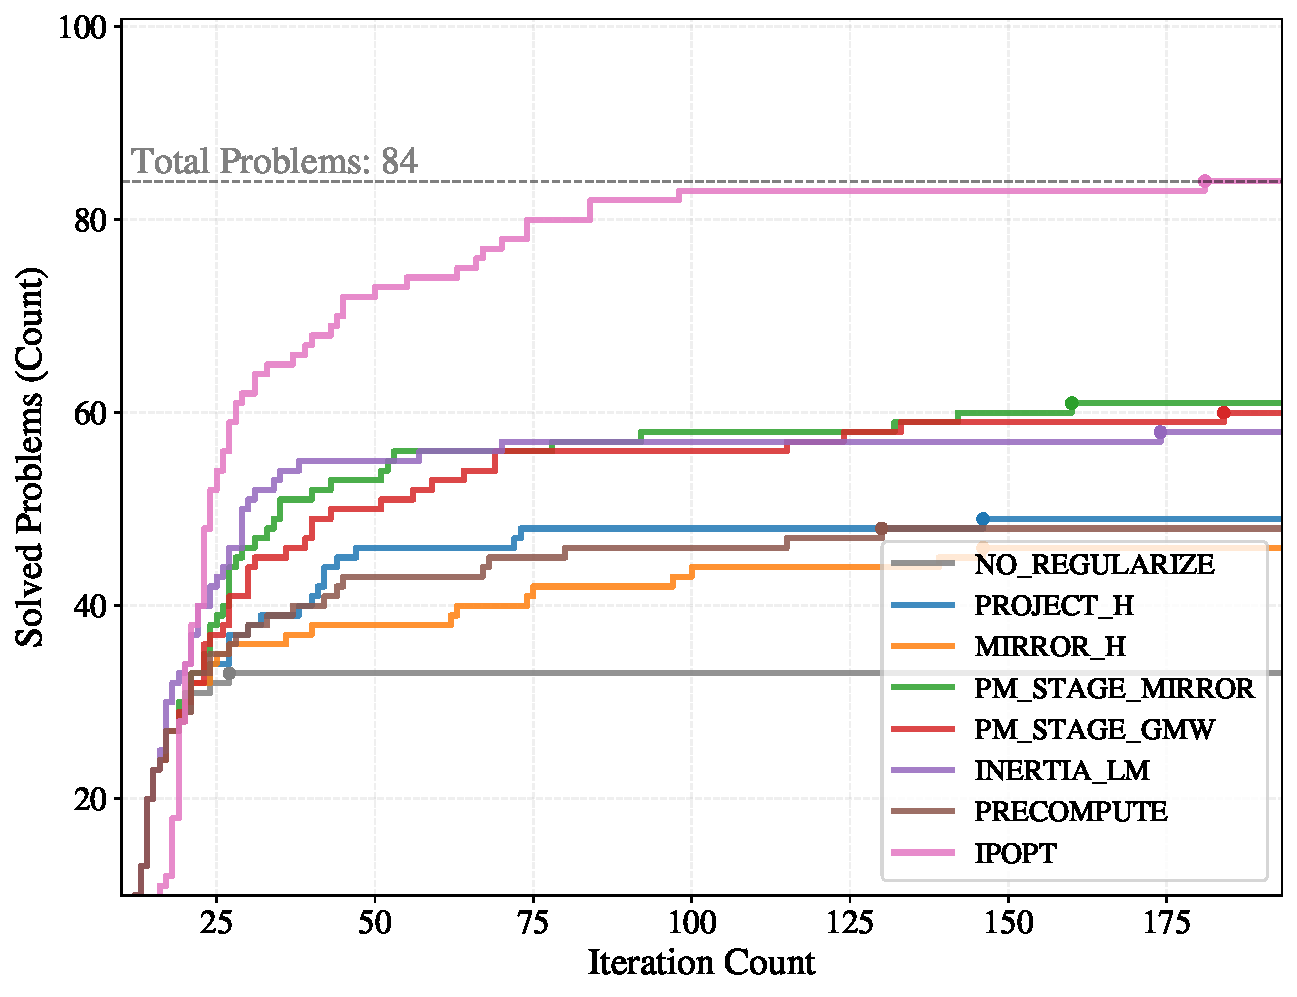
\includegraphics[width=0.7\textwidth]{results/iteration_qp_results_riccati_time_opti.pdf}
    \end{figure}
\end{frame}

\begin{frame}
    \frametitle{Logs in issue: cyclic behavior}
    \begin{table}[htbp]
    \centering
    \footnotesize
    \setlength{\tabcolsep}{4pt}
    \resizebox{\textwidth}{!}{%
    \begin{tabular}{r r r r r r r r r c}
    \toprule
    iter & res\_stat & res\_eq & res\_ineq & res\_comp & duality\_gap & alpha\_prim & alpha\_dual & obj & ls \\
    \midrule
    0  & 1.193190e+02 & 6.562897e-02 & 1.000000e-01 & 1.000000e+01 & 1.000000e+01 & 0.000000e+00 & 0.000000e+00 & 9.085439e-05  & --  \\
    1  & 4.080023e+01 & 8.863925e-03 & 1.350612e-02 & 4.178952e+00 & 3.579625e+00 & 8.649388e-01 & 6.580576e-01 & 1.779560e-01  & 1h  \\
    2  & 6.533249e+00 & 1.027224e-04 & 1.565199e-04 & 9.580696e-01 & 5.872488e-01 & 9.884112e-01 & 8.398722e-01 & 1.996014e-01  & 1h  \\
    3  & 2.525902e-01 & 8.230739e-06 & 1.254132e-05 & 6.039455e-02 & 2.329072e-02 & 9.198739e-01 & 9.613377e-01 & 1.933990e-01  & 1f  \\
    4  & 1.848937e-01 & 6.569681e-06 & 1.001034e-05 & 4.986832e-02 & 1.956711e-02 & 2.018115e-01 & 2.680091e-01 & 1.194161e-01  & 1f  \\
    5  & 1.078514e-01 & 4.343221e-06 & 6.617841e-06 & 3.536902e-02 & 1.426585e-02 & 3.388993e-01 & 4.328154e-01 & -5.572105e-02 & 1f  \\
    6  & 2.266157e-02 & 2.313607e-06 & 3.525283e-06 & 1.520388e-02 & 2.261386e-03 & 4.673062e-01 & 8.678344e-01 & -8.958347e-02 & 1f  \\
    7  & 2.674098e-03 & 1.745698e-08 & 2.659950e-08 & 1.520326e-03 & 2.591079e-04 & 9.924546e-01 & 9.213563e-01 & -1.745445e-01 & 1f  \\
    8  & 9.285079e-04 & 6.421087e-11 & 9.783996e-11 & 2.947232e-04 & 2.123969e-05 & 9.963218e-01 & 9.105802e-01 & -1.897593e-01 & 1f  \\
    $\vdots$ & $\vdots$ & $\vdots$ & $\vdots$ & $\vdots$ & $\vdots$ & $\vdots$ & $\vdots$ & $\vdots$ & $\vdots$ \\
    192 & 9.096204e-06 & 1.283695e-16 & 1.455192e-11 & 4.149841e-07 & 3.886800e-08 & 9.999696e-01 & 9.999988e-01 & -1.907825e-01 & 1f \\
    193 & 2.486766e-04 & 1.056013e-16 & 1.455192e-11 & 4.149841e-07 & 3.886800e-08 & 9.993160e-01 & 9.999991e-01 & -1.907825e-01 & 1f \\
    194 & 2.317297e-04 & 1.331400e-16 & 1.455192e-11 & 4.149841e-07 & 3.886800e-08 & 9.999134e-01 & 9.999103e-01 & -1.907825e-01 & 1f \\
    195 & 2.309347e-05 & 1.548241e-16 & 1.455192e-11 & 4.149841e-07 & 3.886800e-08 & 9.999439e-01 & 9.999221e-01 & -1.907825e-01 & 1f \\
    196 & 1.084048e-05 & 1.999269e-16 & 1.455192e-11 & 4.149841e-07 & 3.886800e-08 & 9.999432e-01 & 9.999823e-01 & -1.907825e-01 & 1f \\
    197 & 1.175446e-05 & 1.782428e-16 & 1.455192e-11 & 4.149841e-07 & 3.886800e-08 & 9.999946e-01 & 9.999797e-01 & -1.907825e-01 & 1f \\
    198 & 1.973085e-04 & 1.331400e-16 & 1.455192e-11 & 4.149841e-07 & 3.886800e-08 & 9.994787e-01 & 9.999992e-01 & -1.907825e-01 & 1f \\
    199 & 5.115843e-06 & 2.658464e-16 & 1.455192e-11 & 4.149841e-07 & 3.886800e-08 & 9.999987e-01 & 9.999823e-01 & -1.907825e-01 & 1f \\
    200 & 1.824212e-05 & 1.222980e-16 & 1.455192e-11 & 4.149841e-07 & 3.886800e-08 & 9.999951e-01 & 9.999606e-01 & 0.000000e+00  & 1f \\
    \bottomrule
    \end{tabular}%
    }
    \label{tab:solver-log}
    \end{table}
\end{frame}

\begin{frame}
    \frametitle{Logs in issue: incorrect direction}
    \begin{table}[htbp]
    \centering
    \footnotesize
    \setlength{\tabcolsep}{4pt}
    \resizebox{\textwidth}{!}{%
    \begin{tabular}{r r r r r r r r r c}
    \toprule
    iter & res\_stat & res\_eq & res\_ineq & res\_comp & duality\_gap & alpha\_prim & alpha\_dual & obj & ls \\
    \midrule
    0   & 9.975000e+01 & 4.245822e-03 & 1.000000e-01 & 1.000000e+01 & 1.000000e+01 & 0.000000e+00 & 0.000000e+00 & 9.417869e-09  & --  \\
    1   & 5.776896e-01 & 1.009637e-04 & 2.377954e-03 & 4.618879e-01 & 5.966625e-02 & 9.762205e-01 & 9.942086e-01 & 3.707784e-03  & 1h  \\
    2   & 5.688686e-02 & 5.279679e-07 & 1.243500e-05 & 1.726627e-02 & 5.354052e-03 & 9.947707e-01 & 9.015287e-01 & 1.201696e-03  & 1f  \\
    3   & 1.285496e-02 & 1.221599e-08 & 2.877179e-07 & 4.594022e-03 & 1.230604e-03 & 9.768622e-01 & 7.740821e-01 & -5.980565e-04 & 1f  \\
    4   & 3.428063e-02 & 1.212721e-08 & 2.856270e-07 & 1.999448e-03 & 1.124835e-03 & 7.267355e-03 & 1.169836e-01 & 7.821219e-04  & 3f  \\
    5   & 4.309372e-02 & 9.883651e-09 & 2.327853e-07 & 1.725207e-03 & 1.135185e-03 & 1.850024e-01 & 3.903366e-02 & -1.965721e-02 & 1f  \\
    6   & 5.200209e-02 & 7.347984e-09 & 1.730639e-07 & 1.635216e-03 & 1.112812e-03 & 2.565516e-01 & 1.011257e-01 & -3.844930e-02 & 1f  \\
    7   & 5.952839e-02 & 6.907065e-09 & 1.626791e-07 & 1.760167e-03 & 1.058101e-03 & 6.000548e-02 & 1.929308e-01 & -3.179804e-02 & 3f  \\
    8   & 4.350804e-02 & 5.670661e-09 & 1.335586e-07 & 1.421848e-03 & 1.024213e-03 & 1.790058e-01 & 1.245698e-01 & -1.201712e-02 & 1h  \\
    9   & 5.011940e-02 & 4.574485e-09 & 1.077409e-07 & 1.397659e-03 & 1.037539e-03 & 1.933065e-01 & 4.597121e-02 & -2.037111e-02 & 1f  \\
    10  & 9.568155e-02 & 4.562375e-09 & 1.074556e-07 & 3.523809e-03 & 8.232296e-04 & 2.647210e-03 & 4.166648e-01 & -2.008499e-02 & 5x  \\
    $\vdots$ & $\vdots$ & $\vdots$ & $\vdots$ & $\vdots$ & $\vdots$ & $\vdots$ & $\vdots$ & $\vdots$ & $\vdots$ \\
    190 & 3.983142e+03 & 4.065758e-16 & 1.455192e-11 & 6.575611e-05 & 3.914307e-06 & 1.527614e-02 & 1.000000e+00 & -4.940286e-02 & 2f \\
    191 & 2.984527e+02 & 2.810252e-16 & 1.000009e-12 & 6.612608e-05 & 2.473030e-06 & 2.955980e-01 & 9.250710e-01 & -4.937099e-02 & 1h \\
    192 & 2.590495e+02 & 5.276947e-16 & 1.455192e-11 & 6.641365e-05 & 2.685206e-06 & 8.274469e-02 & 1.320251e-01 & -4.951826e-02 & 1f \\
    193 & 2.532566e+02 & 4.347786e-16 & 1.455192e-11 & 6.646826e-05 & 2.721274e-06 & 3.466426e-02 & 2.236196e-02 & -4.951540e-02 & 1f \\
    194 & 1.765414e+01 & 5.041405e-16 & 1.000007e-12 & 6.827519e-05 & 3.540048e-06 & 5.844196e-02 & 1.000000e+00 & -4.952119e-02 & 1f \\
    195 & 7.560961e-01 & 5.383877e-16 & 1.455192e-11 & 6.896862e-05 & 2.710779e-06 & 3.124999e-02 & 1.000000e+00 & -4.952004e-02 & 5x \\
    196 & 1.168906e+00 & 4.742114e-16 & 1.000006e-12 & 7.021518e-05 & 3.163520e-06 & 8.392660e-02 & 1.000000e+00 & -4.951324e-02 & 1h \\
    197 & 1.820370e+00 & 3.604837e-16 & 1.455192e-11 & 7.021723e-05 & 2.223239e-06 & 9.524931e-01 & 7.993635e-01 & -4.960680e-02 & 1f \\
    198 & 1.823966e+00 & 4.139670e-16 & 1.000000e-12 & 7.021835e-05 & 2.247188e-06 & 6.249999e-02 & 6.478533e-04 & -4.951209e-02 & 5f \\
    199 & 1.396138e+02 & 4.816026e-16 & 1.455192e-11 & 7.062518e-05 & 2.546685e-06 & 1.232371e-01 & 2.756777e-01 & -4.955614e-02 & 1f \\
    200 & 1.395517e+02 & 4.925818e-16 & 1.455192e-11 & 7.062627e-05 & 2.547619e-06 & 6.528403e-04 & 4.443489e-04 & 0.000000e+00  & 2f \\
    \bottomrule
    \end{tabular}%
    }
    \label{tab:solver-log}
    \end{table}
\end{frame}


\begin{frame}
    \frametitle{Some possible next steps}
    \begin{itemize}
        \item Theoretical parts for:
        \begin{itemize}
            \item Why Mehrotra probing works better than predictor-corrector on indefinite QPs
            \item Why PROJECT, MIRROR, PRECOMPUTE fails
            \item Pros and cons of PM\_STAGE\_MIRROR, PM\_STAGE\_GMW over INERTIA\_CORRECTION
        \end{itemize}
        \item Engineering parts on:
        \begin{itemize}
            \item Collecting more indefinite QPs?
            \item More Methods?
            \item implementations?
        \end{itemize}
    \end{itemize}
\end{frame}

\begin{frame}
    \frametitle{FYI: with Mehrotra predictor-corrector on convex QPs}
    \begin{figure}
        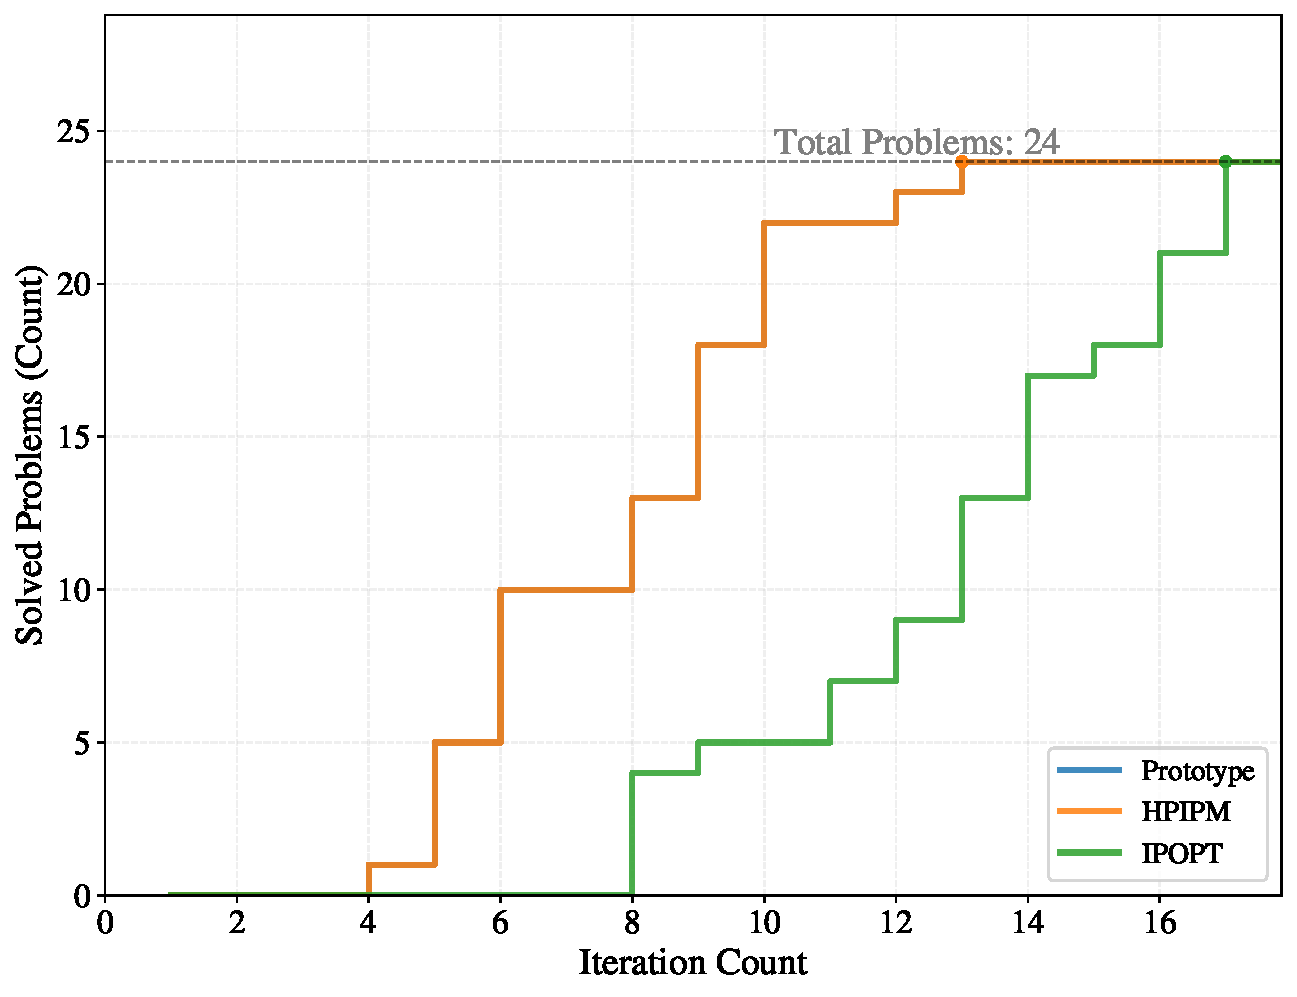
\includegraphics[width=0.7\textwidth]{results/iteration_qp_results_pos.pdf}
    \end{figure}
\end{frame}

\begin{frame}
    \frametitle{FYI: with Mehrotra predictor-corrector on indefinite QPs}
    \begin{figure}
        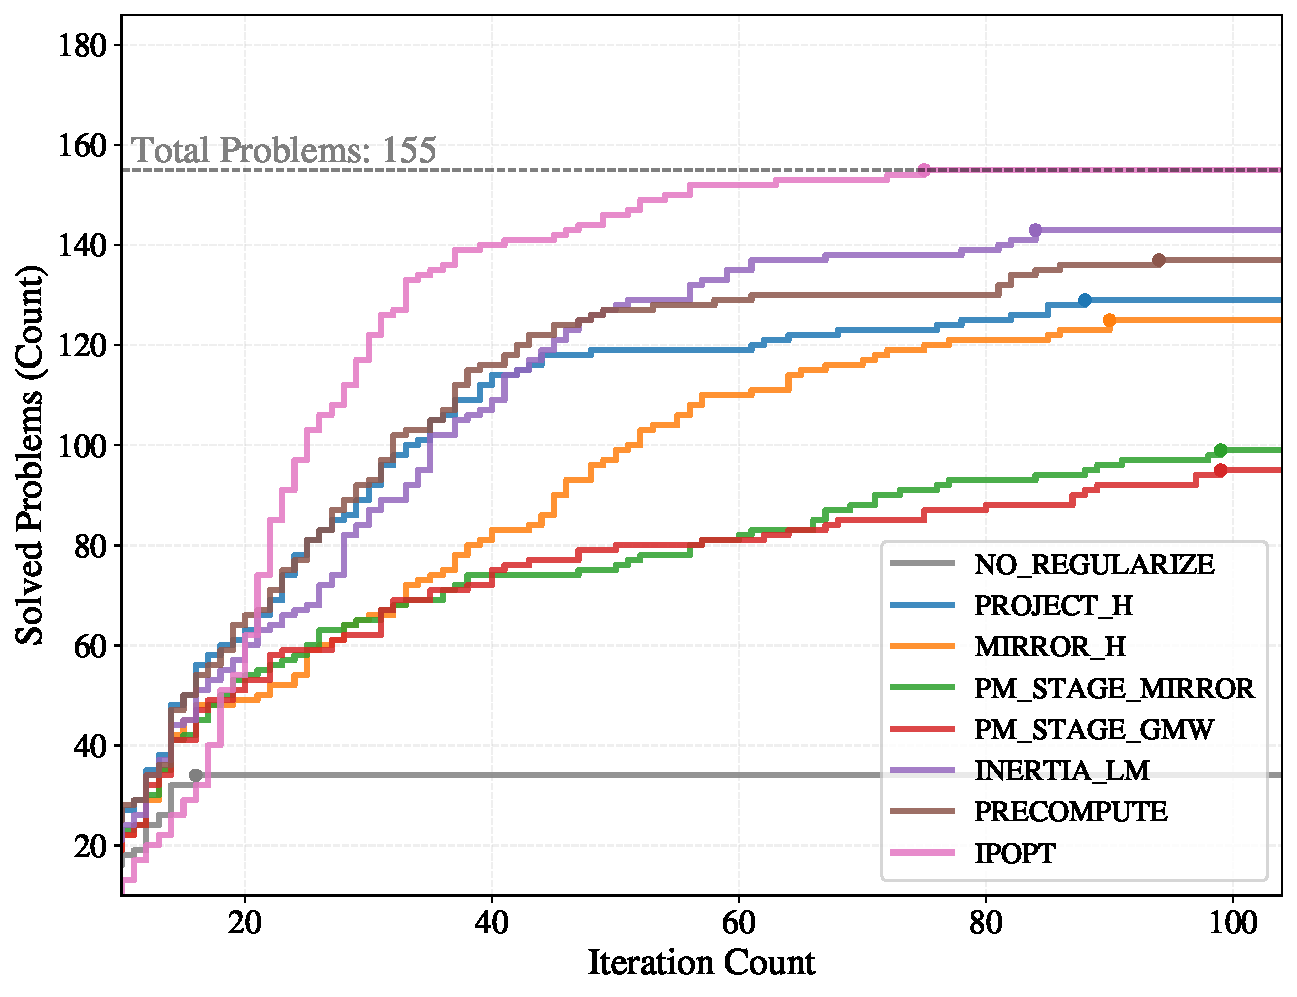
\includegraphics[width=0.7\textwidth]{results/iteration_qp_results_riccati_pc.pdf}
    \end{figure}
\end{frame}

\begin{frame}
    \frametitle{FYI: with Mehrotra predictor-corrector on indefinite QPs}
    \begin{figure}
        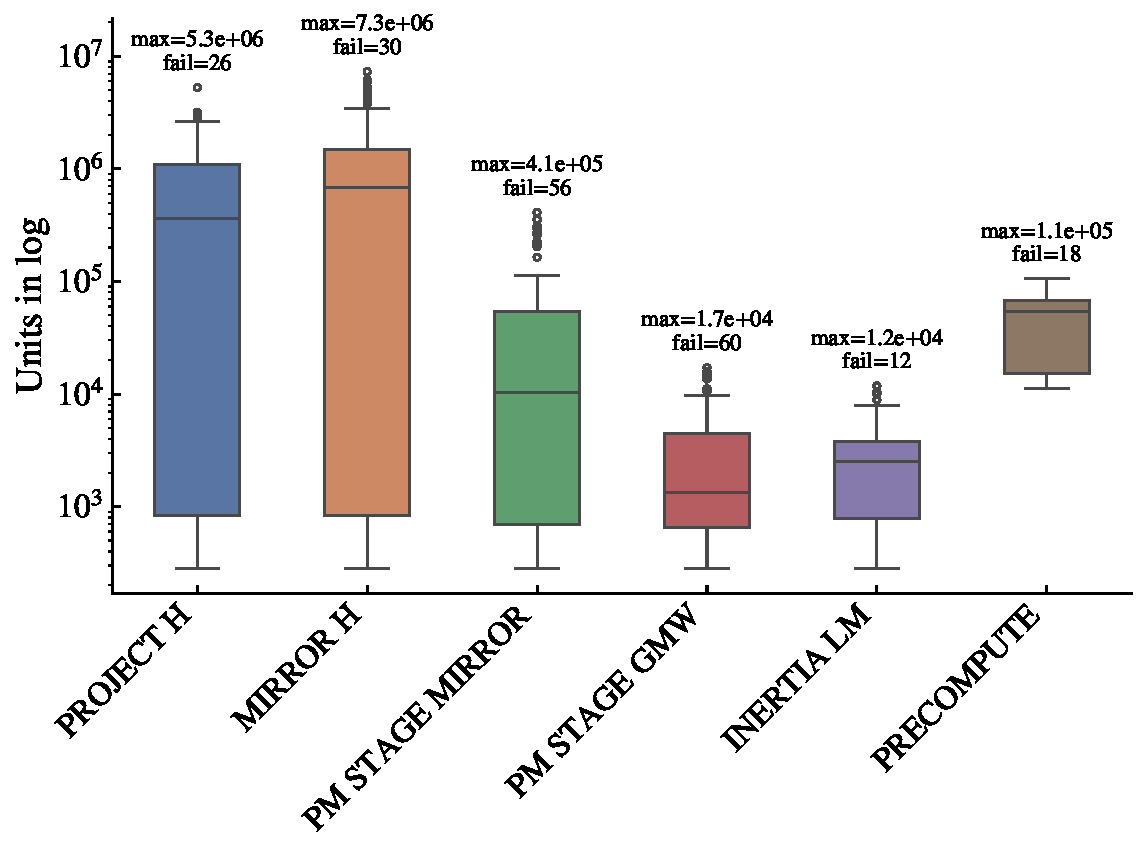
\includegraphics[width=0.7\textwidth]{results/decomp_flop_worstcase_qp_results_riccati_pc.pdf}
    \end{figure}
\end{frame}


\begin{frame}
    \frametitle{FYI: without funnel line search on indefinite QPs}
    \begin{figure}
        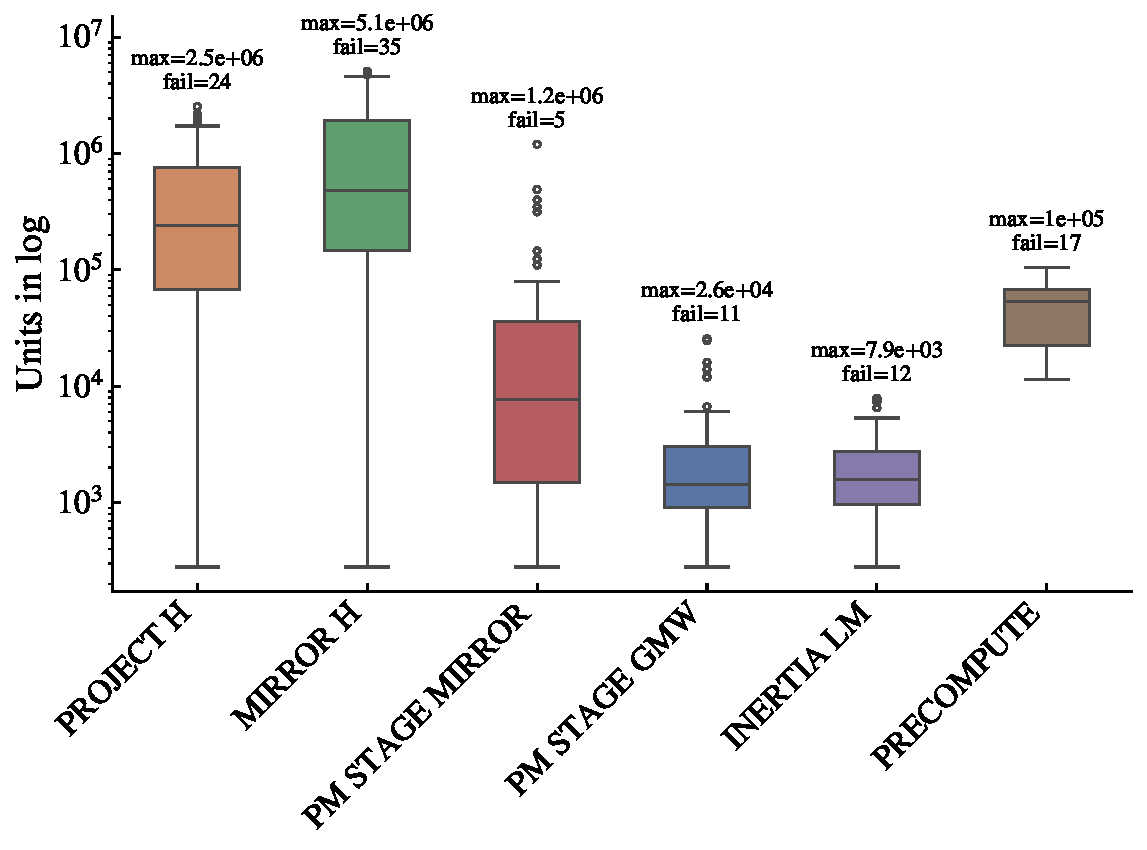
\includegraphics[width=0.7\textwidth]{results/decomp_flop_worstcase_qp_results_riccati_nosearch.pdf}
    \end{figure}
\end{frame}


\bibliographystyle{IEEEtran}
\bibliography{references}

\end{document}
